% P is deliberately not the incenter. A=(5,12),B=(0,0),C=(14,0),P=(6,5).
\begin{center}
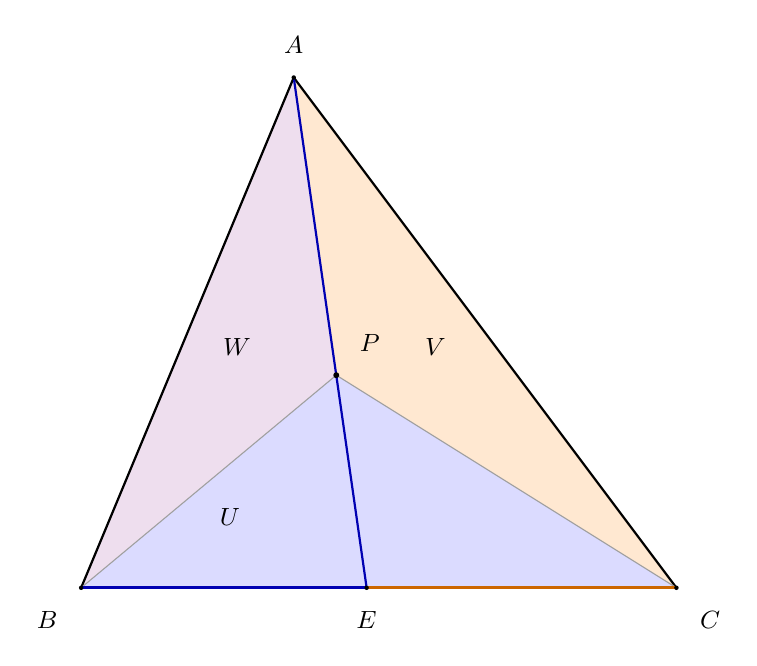
\begin{tikzpicture}[scale=.54,font=\small,line cap=round,line join=round]
\coordinate (A) at (5,12);\coordinate (B) at (0,0);\coordinate (C) at (14,0);
\coordinate (P) at (6,5);\coordinate (E) at (47/7,0);
\fill[blue!14] (P)--(B)--(C)--cycle;
\fill[orange!18] (P)--(C)--(A)--cycle;
\fill[violet!13] (P)--(A)--(B)--cycle;
\draw[thick] (A)--(B)--(C)--cycle;
\draw[gray!75] (P)--(B) (P)--(C);
\draw[thick,blue!70!black] (A)--(E);
\draw[blue!70!black,very thick] (B)--(E);
\draw[orange!80!black,very thick] (E)--(C);
\node at (3.5,5/3) {$U$};
\node at (25/3,17/3) {$V$};\node at (11/3,17/3) {$W$};
\foreach \Q/\pos in {A/above,B/below left,C/below right,E/below}{\fill (\Q) circle[radius=1.5pt];\node[\pos=5pt] at (\Q) {$\Q$};}
\fill (P) circle[radius=2pt];\node[above right=5pt] at (P) {$P$};
\end{tikzpicture}
\par\smallskip{\small $P$ 是任意内点；同高给出 $BE:EC=W:V$，同底给出 $PE:AE=U:(U+V+W)$。}
\end{center}
